

We here rely on axisymmetric cylindrical coordinates, see Section~\ref{MMM-ss:axicyleqs}.
As shown on the following figure we assume that the deformation/flow is independent of the angle 
$\theta$ so that the remaining space coordinates are $r$ and $z$.
\begin{center}
\begin{flushright} {\tiny {\color{gray} (tikz\_axi.tex)}} \end{flushright}
%~~~~~~~~~~~~~~~~~~~~~~~~~~~~~~~~~~~~~~~~~~~~~~~~~~~~~~~~~~~~~~~~~~~~~~~~~~~~~~~~~~~~~~~~~~~~~~~~~~

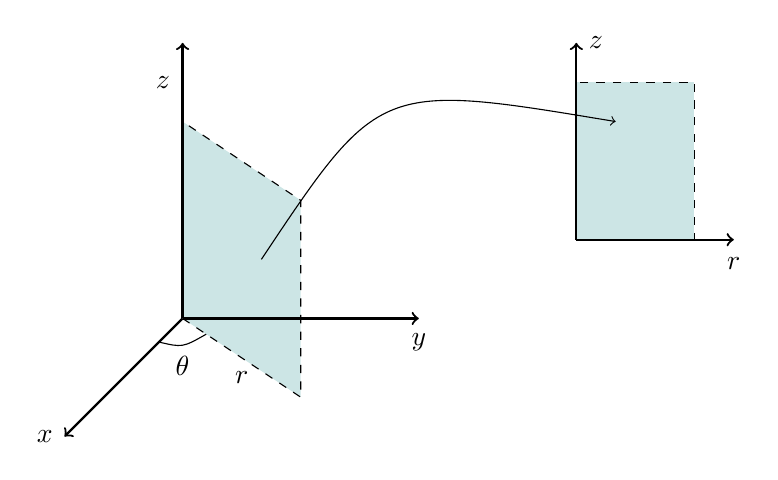
\begin{tikzpicture}
%\draw[step=0.5cm,gray,very thin] (0,0) grid (10,6); %background grid

\draw[dashed,fill=teal!20] (2,2)--(3.5,1)--(3.5,3.5)--(2,4.5)--cycle ;
\draw[thick,->] (2,2) -- (0.5,0.5); 
\draw[thick,->] (2,2) -- (5,2); 
\draw[thick,->] (2,2) -- (2,5.5); 
\node[] at (0.25,0.5) {$x$};
\node[] at (5,1.7) {$y$};
\node[] at (1.75,5) {$z$};
\node[] at (2.75,1.25) {$r$};
\node[] at (2,1.4) {$\theta$};
\draw[] (1.7,1.7) .. controls (2,1.63) ..   (2.3,1.8);

\draw[dashed,fill=teal!20] (7,3)--(8.5,3)--(8.5,5)--(7,5)--cycle; 
\draw[thick,->] (7,3) -- (9,3); 
\draw[thick,->] (7,3) -- (7,5.5); 
\node[] at (9,2.7) {$r$};
\node[] at (7.25,5.5) {$z$};

\draw[->] (3,2.75) .. controls (4.5,5) .. (7.5,4.5);
\end{tikzpicture}



\end{center}

Given the symmetry of the problem any term containing $\partial_\theta$ or $\upnu_\theta$ is zero.
The strain rate tensor given in Section~\ref{MMM-ss:srcc} then simplifies to:

\begin{eqnarray}
\dot\varepsilon_{rr} 
&=& \frac{\partial \upnu_r}{\partial r} \nn\\
\dot\varepsilon_{\theta\theta}  &=& \frac{\upnu_r}{r} \nn\\
\dot\varepsilon_{\theta r} = \dot\varepsilon_{r\theta}  &=& 0 \nn\\
\dot\varepsilon_{zz} &=& \frac{\partial \upnu_z}{\partial z} \nn\\
\dot{\varepsilon}_{rz} = \dot{\varepsilon}_{zr} 
&=& \frac{1}{2}\left( \frac{\partial \upnu_r}{\partial z} + \frac{\partial \upnu_z}{\partial r} \right) \nn\\
\dot{\varepsilon}_{\theta z} = \dot{\varepsilon}_{z \theta} &=& 0 \nn
\end{eqnarray}
Note that the term $\dot\varepsilon_{\theta\theta} $ is not zero!
The deviatoric stress tensor ${\bm \tau}=2\eta \dot{\bm \varepsilon}$ can be computed
as well as the full stress tensor ${\bm \sigma}=-p {\bm 1} + {\bm \tau}$. 


In cylindrical coordinates, and in the axisymmetric case
the strain rate tensor is given by
\[
\dot{\bm\varepsilon}(\vec\upnu)
=
\left(
\begin{array}{ccc}
\dot\varepsilon_{rr} & 0 & \dot{\varepsilon}_{rz} \\
0 & \dot{\varepsilon}_{\theta\theta}  & 0 \\
\dot{\varepsilon}_{zr} & 0 & \dot\varepsilon_{zz}
\end{array}
\right)
\]
